\documentclass{article}
\usepackage{tikz, comment}
\usepackage{pifont}
\usepackage{fontspec}
\usetikzlibrary{arrows, decorations.markings, decorations.pathreplacing}
\begin{comment}
:Title: Not defined yet
:Slug: No name yet

Description Here.........
\end{comment}
\begin{document}\centering 

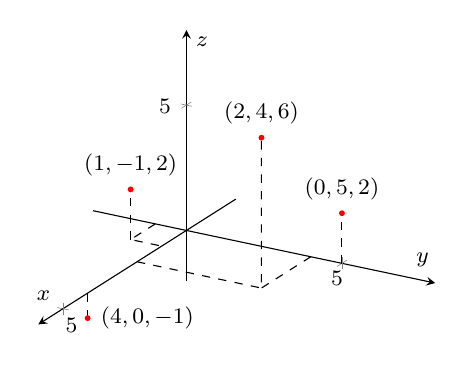
\begin{tikzpicture}[font=\footnotesize]
\pgfplotsset{compat=1.8}
\begin{axis}
[axis lines = center, view={120}{30},
axis on top, xlabel = {$x$}, ylabel ={$y$}, zlabel ={$z$}, domain =0:1, y domain =0:1,
xmin =-2.0,
xmax =6.0,
ymin =-3.0,
ymax =8,
zmin =-2.0, 
zmax =8.0,
samples =10, samples y =40, z buffer =sort]

\addplot3[dashed] coordinates
        {(1,-1,2) (1,-1,0)};
\node[label={90:{$(1,-1,2)$}},circle,fill=red,inner sep=0.75pt] at (axis cs:1,-1,2) {};
\addplot3[dashed] coordinates
        {(1,0,0) (1,-1,0) (0,-1,0)};

\addplot3[dashed] coordinates
        {(2,4,6) (2,4,0) (2,0,0)};
\node[label={90:{$(2,4,6)$}},circle,fill=red,inner sep=0.75pt] at (axis cs:2,4,6) {};
\addplot3[dashed] coordinates
        {(2,4,0) (0,4,0)};

\addplot3[dashed] coordinates
        {(4,0,-1) (4,0,0)};
\node[label={0:{$(4,0,-1)$}},circle,fill=red,inner sep=0.75pt] at (axis cs:4,0,-1) {};

\addplot3[dashed] coordinates
        {(0,5,2) (0,5,0)};
\node[label={90:{$(0,5,2)$}},circle,fill=red,inner sep=0.75pt] at (axis cs:0,5,2) {};

\end{axis}

\end{tikzpicture}
\end{document}